\documentclass{beamer}

\usetheme{Boadilla}
\usepackage{natbib}

\title{Variation in Political News}
\subtitle{An NLP Approach}
\author{Stephen Lee}
\institute{University of Memphis}

\begin{document}
	
%%%%%%%%%%%%%%%%%%%%%%%%%%%%%%%%%%%%%%%%%%%%%%%%
% TITLE SLIDES

	\begin{frame}
		\maketitle
	\end{frame}

    \begin{frame}
    	\frametitle{Outline}
    	\tableofcontents
    \end{frame}

%%%%%%%%%%%%%%%%%%%%%%%%%%%%%%%%%%%%%%%%%%%%%%%%
% INTRO

\section{Introduction}

    \subsection{Background}
   
    \begin{frame}
   	    \frametitle{Background}
   	    \begin{center}
   	    	\textit{``If you can't measure it, you can't improve it.''}
   	    \end{center}
   	    \begin{flushright}
   	    	--- Peter Drucker
   	    \end{flushright}
       
       \begin{itemize}
       	\item The 2016 United States Presidential Election raised doubts for many about the quality of their news.
       	\item \citet{allcott2017social} estimate that the average US adult read and remembered about one, and possibly up to several, fake news articles during the election period.
       	\item It is now not uncommon for the president of the United States to tweet that certain news sources are "Fake News". 
       \end{itemize}
    \end{frame}
   
	\subsection{Literature Review}
	
	\begin{frame}
		\frametitle{Literature Review: Computer Science}
		\begin{itemize}
			\item The LSTM architecture was introduced in \citet{hochreiter1997long}. It builds on the Recurrant Neural Network (RNN) architecture to improve lagged information storage for the purpose of processing sequential data.
			\item More recently, \citet{gers2000recurrent}, \citet{chung2014empirical}, and \citet{yao2015depth} introduce variations on the baseline \citet{hochreiter1997long} LSTM model, although \citet{greff2016lstm} show them all to be roughly equivalent on a variety of prediction tasks. 
			\item \citet{schuster1997bidirectional} introduced the first bidirectional RNN reporting a significant predictive improvements over traditional RNNs. Together, bidirectional LSTM architectures prove to be among the most accurate models for language tasks, consistent with \citet{wang2015unified}. 
		\end{itemize}
	\end{frame}
	
	\begin{frame}
		\frametitle{Literature Review: Economics}
		\begin{itemize}
			\item \citet{gentzkow2010drives} find that readers prefer to consume ``like-minded'' news and that the profit maximizing response from news companies can account for around 20\% of the variation in political slant or bias.
			\item \citet{gentzkow2006media} also find that a Bayesian consumer will reinforce their beliefs of a given news source quality when they read something that confirms their priors.
			\item Together, these works suggest that political news bias may tactical, and that this polarization we see may be self-reinforcing.
			\item \citet{gentzkow2008competition} go as far as to suggest that competition in information markets may actually be counterproductive in achieving balanced and unbiased news. 
		\end{itemize}
	\end{frame}

    \subsection{Summary}
    
    \begin{frame}
    	\frametitle{Summary}
    	\begin{itemize}
    		\item With a goal of classifying articles by their news source, I scraped several thousand news articles from Fox, Vox, and PBS News.
    		\item I find that a relatively simple, bidirectional, LSTM recurrent neural network can  correctly predict the source of an article with very high accuracy. 
    		\item I then use the result of this trained network to build a web app that can allow for a copy-and-paste interface to interact with this classification model. 
    		\item To my knowledge, this work provides the first look at news classification using neural networks. 
    	\end{itemize}
    \end{frame}

%%%%%%%%%%%%%%%%%%%%%%%%%%%%%%%%%%%%%%%%%%%%%%%%
% DATA 

\section{Data}

    \begin{frame}
    	\frametitle{Data}
    	\begin{itemize}
    		\item I mined political news articles from the websites of Fox News, Vox News, and PBS News. 
    		\item Intuitively, the motivation is to focus only on sentiment or semantics, rather than subject matter differences.
    		\item By some estimations,\footnote{Source: https://www.adfontesmedia.com.} these three news sites represent distinct categories of news: 
    		\begin{itemize}
    			\item Fox as a conservative “right” opinion. 
    			\item PBS as the “center” primary source news position. 
    			\item Vox as a liberal “left” opinion.
    		\end{itemize} 
    	\end{itemize}
    \end{frame}

    \begin{frame}
    	\begin{figure}[H]
    		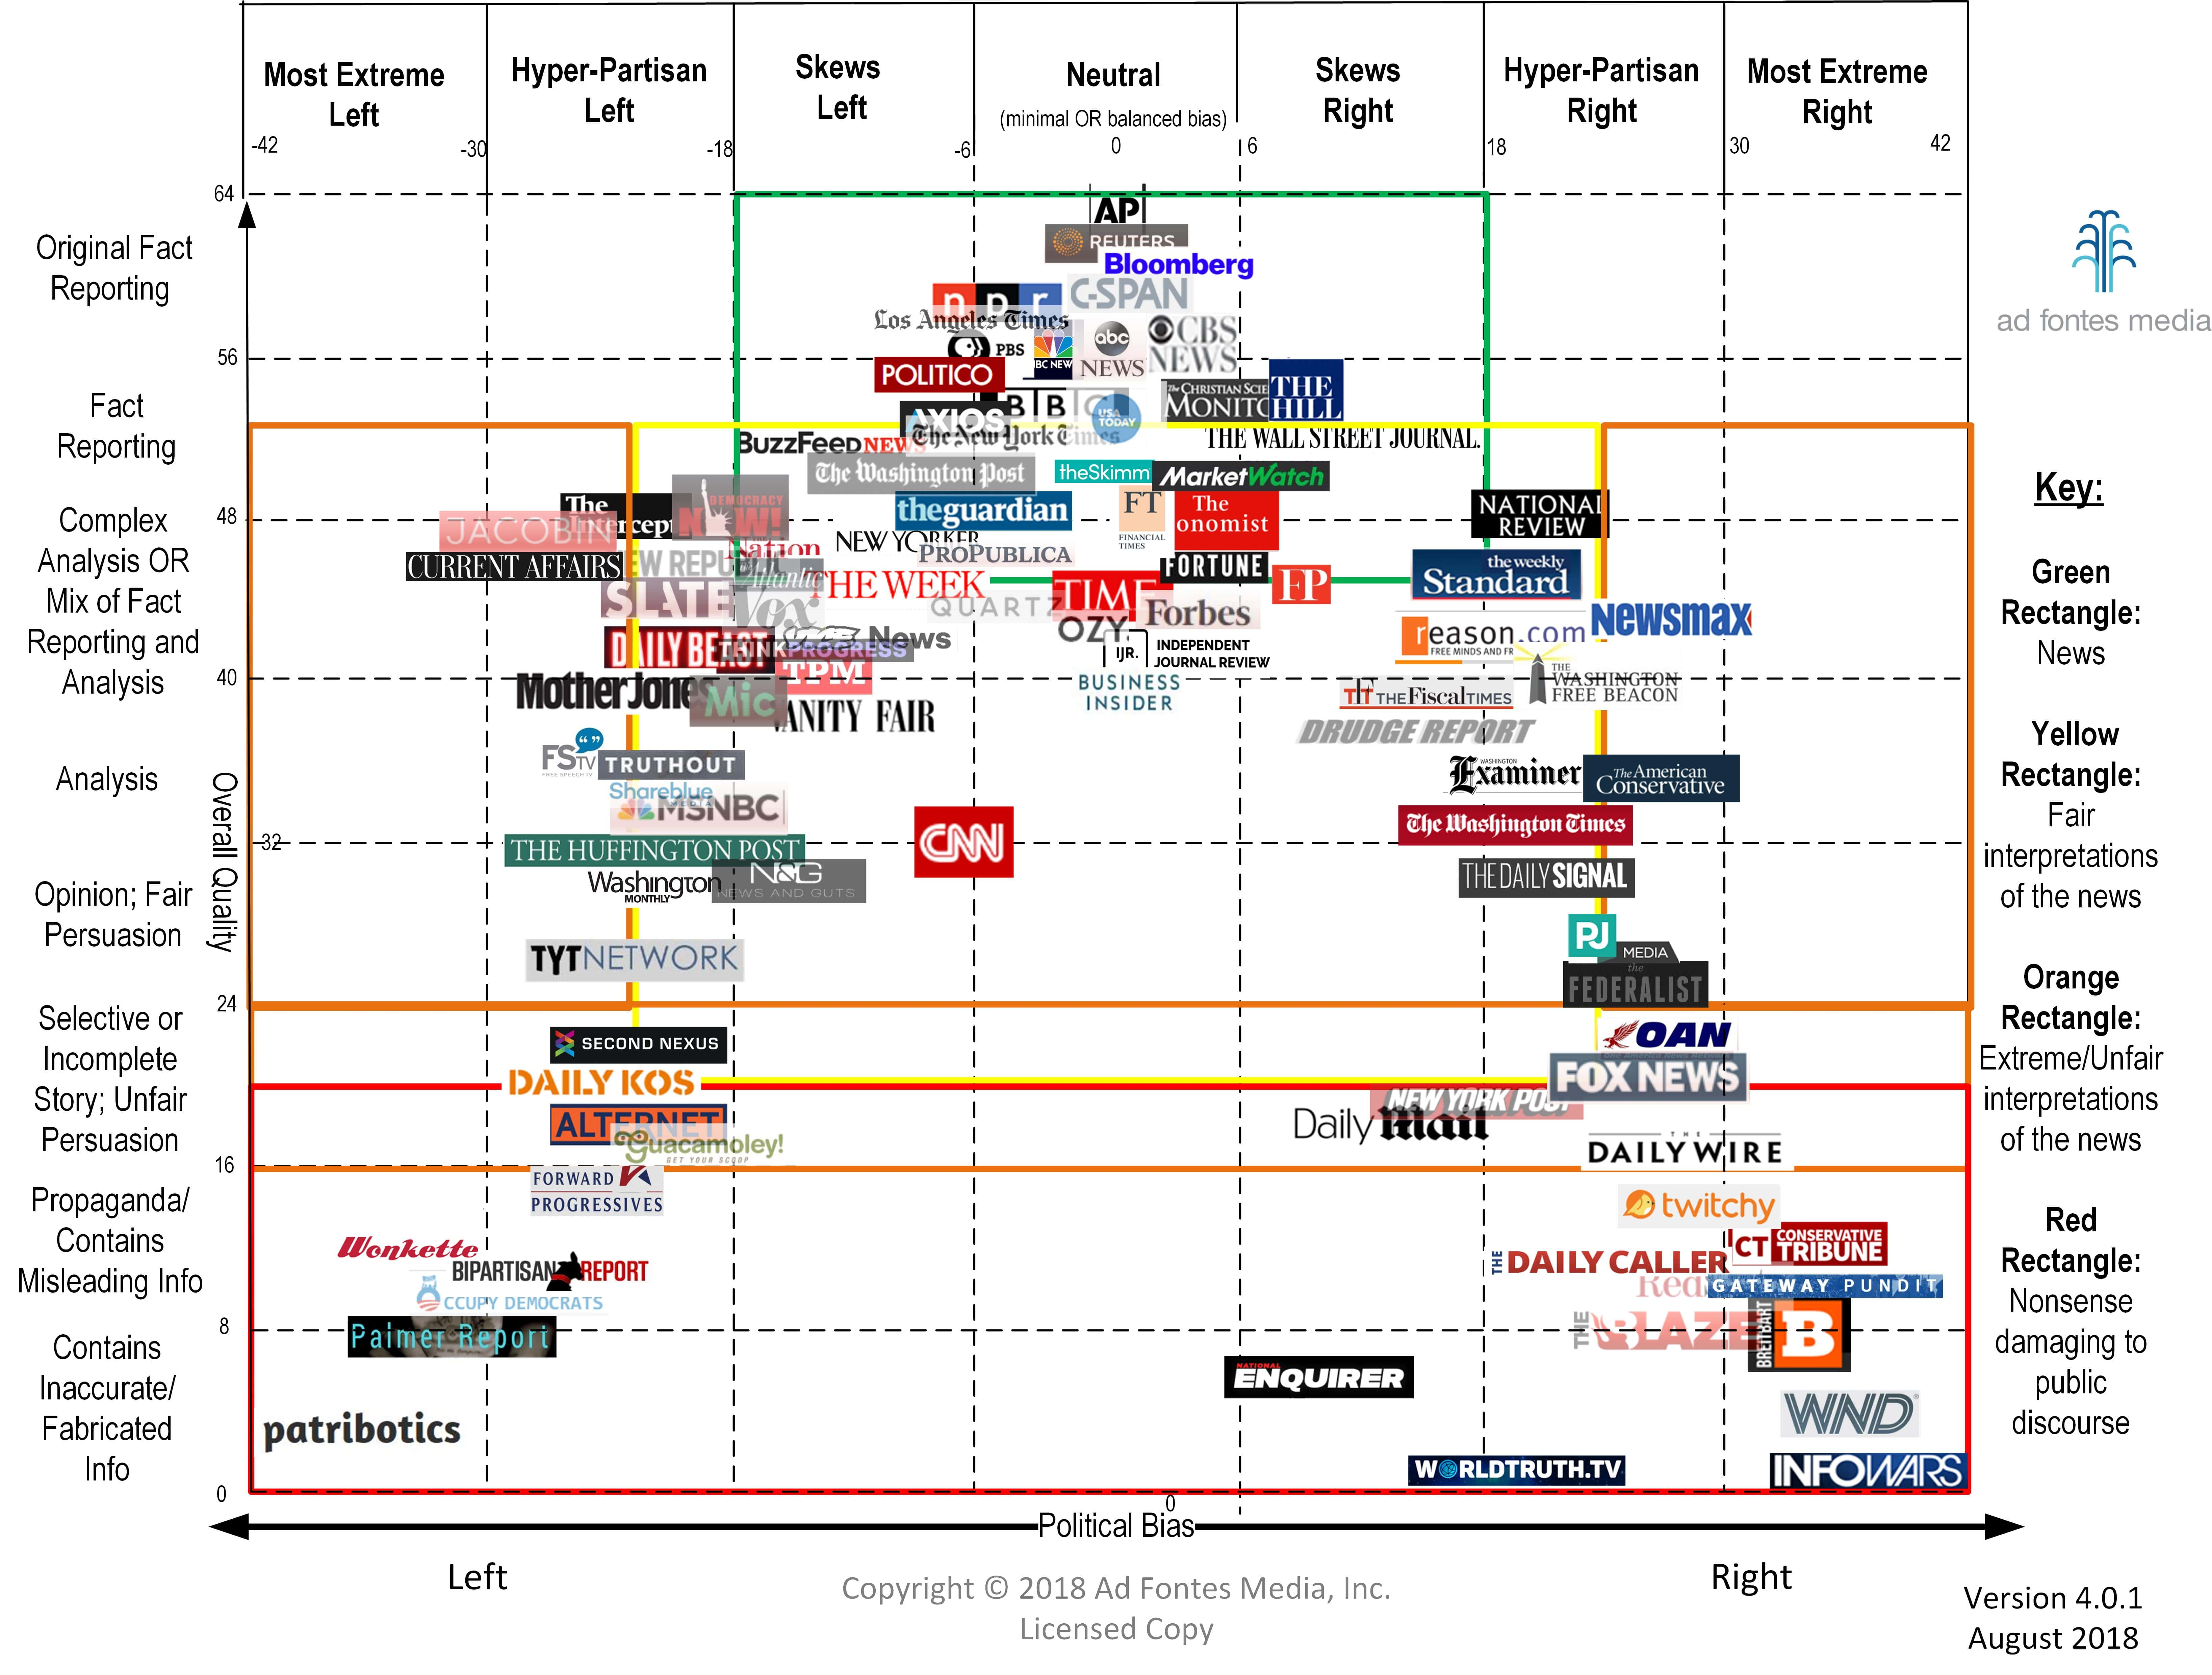
\includegraphics[width=\textwidth]{figures/images/news-bias.jpg}
    		\caption{A graphical depiction of the bias in various political news sources.}
    		\label{fig:news-bias}
    	\end{figure}
    \end{frame}

	\begin{frame}
		\frametitle{Descriptive Statistics}
		\begin{table}[H]
    \centering
    \begin{tabular}{|l|r|r|r|r|r|} \hline
             &                                &                                 &                                       &                                        &                                            \\
             &                                & \multicolumn{1}{c|}{Avg}        &                                       &                                        & \multicolumn{1}{c|}{Avg words}             \\
    Source   & \multicolumn{1}{c|}{Documents} & \multicolumn{1}{c|}{word count} & \multicolumn{1}{c|}{Pct Adjectives}   & \multicolumn{1}{c|}{Pct Adverbs}       & \multicolumn{1}{c|}{per sentence}          \\ \hline \hline
    Fox      & 661                            & 686.2                           & 0.066                                 & 0.034                                  & 20.1                                       \\
    PBS      & 1739                           & 654.3                           & 0.066                                 & 0.032                                  & 18.0                                       \\
    Vox      & 1027                           & 1332.8                          & 0.073                                 & 0.046                                  & 21.3                                       \\ \hline  
    \end{tabular}
    \caption{Summary statistics by data by source. }
    \label{tab:summary}
\end{table}
	\end{frame}

	\begin{frame}
		\frametitle{N-gram Frequencies}
		\begin{table}[H]
    \centering
    \caption{Word Frequencies}
    \label{tab:1gram}
    \begin{tabular}{l|l|l|l} \hline
    \textbf{Num} & \textbf{Vox} & \textbf{PBS} & \textbf{Fox} \\ \hline \hline
    &&& \\
    1   & trump       & trump     & trump      \\
    2   & tax         & said      & said       \\
    3   & will        & president & president  \\
    4   & people      & house     & house      \\
    5   & health      & will      & new        \\
    6   & bill        & new       & will       \\
    7   & republicans & white     & democratic \\
    8   & one         & senate    & democrats  \\
    9   & new         & democrats & told       \\
    10  & care        & campaign  & border     \\ \hline
    \end{tabular}
\end{table}
	\end{frame}

	\begin{frame}
		\frametitle{N-gram Frequencies}
		\begin{table}[H]
    \centering
    \caption{Top frequencies of two word phrases.}
    \label{tab:2gram}
    \begin{tabular}{l|lr|lr|lr}
    \hline
    \textbf{Num} & \multicolumn{2}{c|}{\textbf{Vox}}           & \multicolumn{2}{c|}{\textbf{PBS}}          & \multicolumn{2}{c}{\textbf{Fox}} \\ \hline \hline
    &&&&&& \\
    1   & health care          & 1654 & white house        & 1683 & white house     & 556 \\
    2   & white house          & 743  & president donald   & 1297 & new york        & 359 \\
    3   & trump administration & 672  & donald trump       & 1035 & president trump & 318 \\
    4   & donald trump         & 598  & special counsel    & 613  & green new       & 256 \\
    5   & tax cuts             & 479  & supreme court      & 584  & health care     & 160 \\
    6   & health insurance     & 479  & attorney general   & 499  & new deal        & 151 \\
    7   & new york             & 470  & new york           & 491  & united states   & 134 \\
    8   & affordable care      & 437  & justice department & 485  & border security & 132 \\
    9   & tax bill             & 376  & counsel robert     & 405  & donald trump    & 131 \\
    10  & federal government   & 365  & trump said         & 369  & state union     & 126 \\ \hline
    \end{tabular}
\end{table}
	\end{frame}

    \subsection{Challenges}
    
    \begin{frame}
    	\frametitle{Challenges}
		\begin{enumerate}
			\item Difference in corpus size from each source. 
			\begin{itemize}
				\item Bootstrap the data. 
			\end{itemize}  
		
		    \item Variability of online formatting. 
		    \begin{itemize}
		    	\item I removed any mention of their own organization.
		    	\item Other common and unique affiliations. 
		    	\item Any other noticeable identifying characteristics.
		    \end{itemize}   
	    
	        \item Difference in the average article length. 
	        \begin{itemize}
	        	\item I limited the article length to the first 500 words.
	        \end{itemize}
		\end{enumerate}
    \end{frame}
    

%%%%%%%%%%%%%%%%%%%%%%%%%%%%%%%%%%%%%%%%%%%%%%%%
% STATISTICAL ANALYSIS 

\section{Statistical Analysis}
	
%%%%%%%%%%%%%%%%%%%%%%%%%%%%%%%%%%%%%%%%%%%%%%%%
% NEURAL NETWORK MODEL

\section{LSTM Model}

    \begin{frame}
    	\frametitle{LSTM Model}
    	\begin{figure}[H]
    		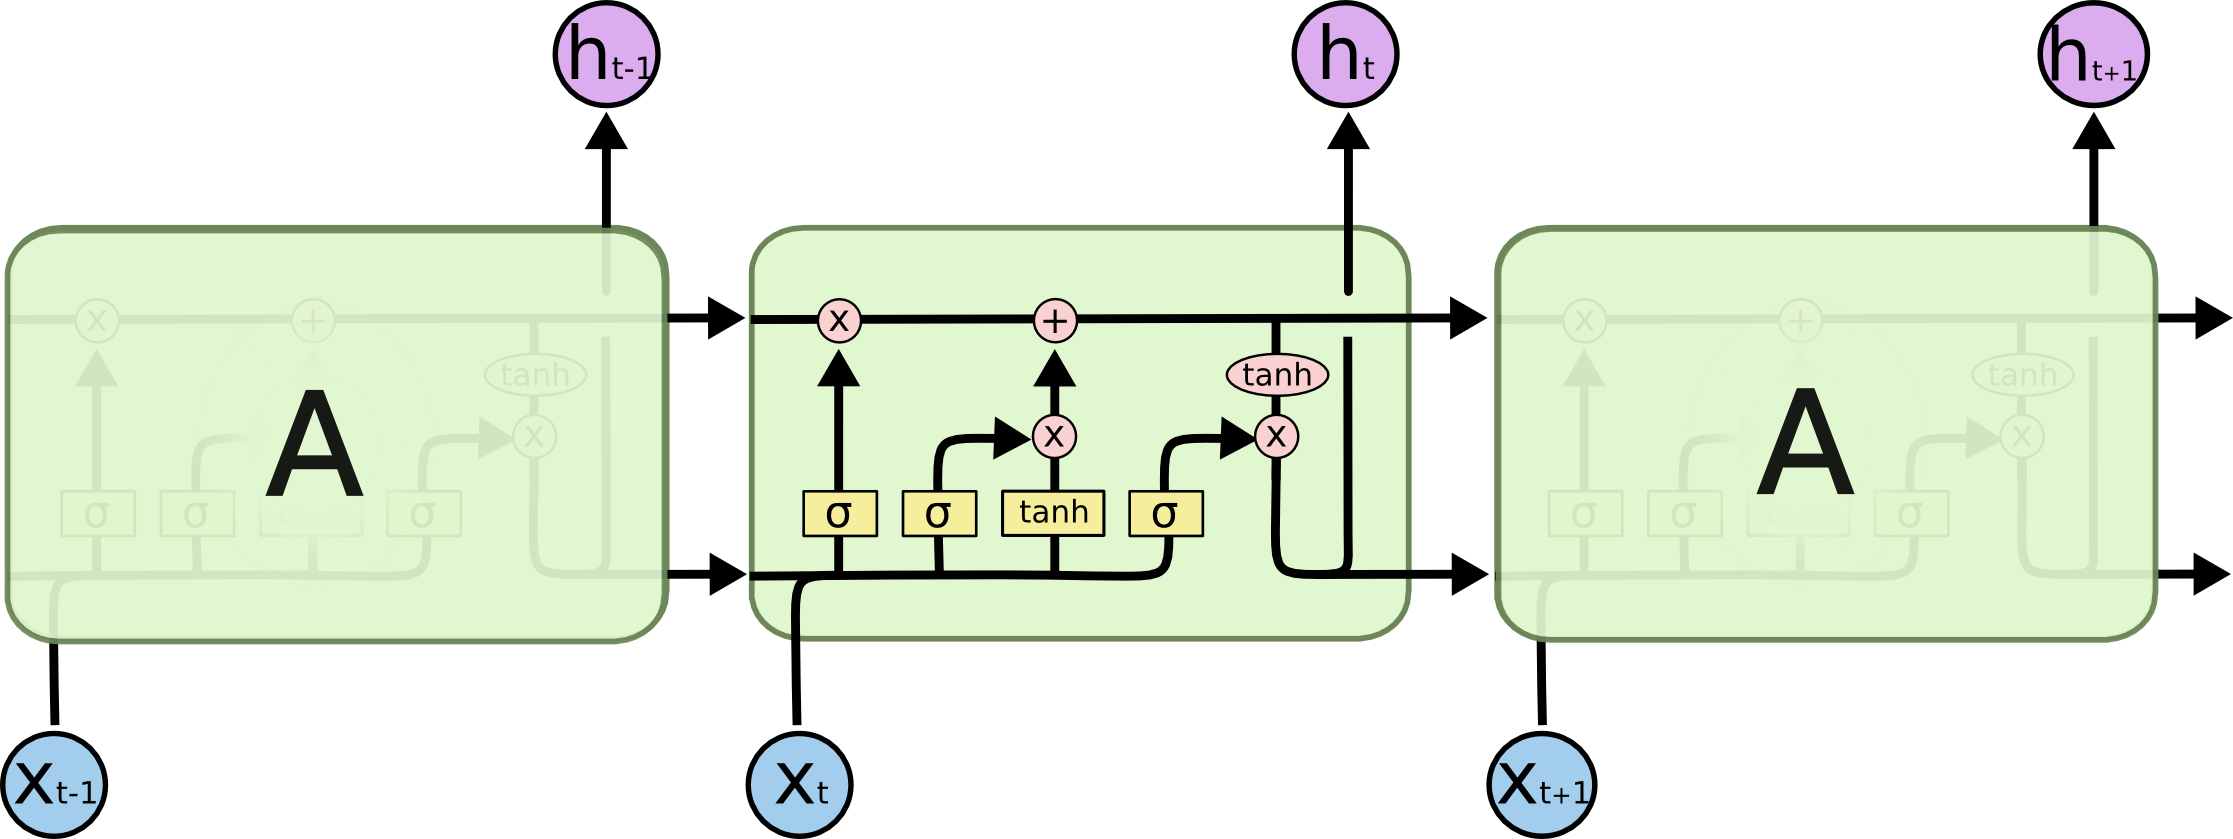
\includegraphics[width=\textwidth]{figures/images/lstm-math.png}
    		\caption{A graphical depiction of a single LSTM cell.\footnote{Source: https://colah.github.io/posts/2015-08-Understanding-LSTMs}}
    	\end{figure}
    \end{frame}

    \begin{frame}
    	\frametitle{Bidirectional Training}
    	\begin{figure}[H]
    		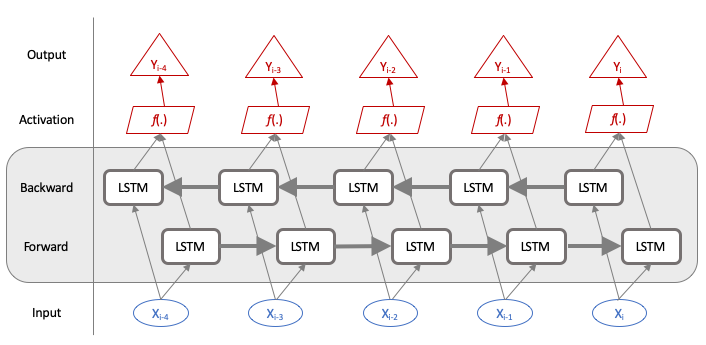
\includegraphics[width=\textwidth]{figures/images/bidirectional-net.png}
    		\caption{A visual representation of a bidirectional LSTM training.}
    	\end{figure}
    \end{frame}

    \begin{frame}
    	\frametitle{Word Embedding}
    	\begin{itemize}
    		\item I use the common crawl 840B Global Word Vector (i.e. GloVe).
    		\item Introduced in \citet{pennington2014glove} and uses 840 billion tokens and a case-sensitive vocabulary of 2.2 million words to map words into a corresponding $300 \times 1$ dimensional vector. 
    		\item Accordingly, I do minimal preprocessing to the text besides the basic cleaning mentioned previously. 
    	\end{itemize}
    \end{frame}

    \begin{frame}
    	\frametitle{Methodology}
    	\begin{itemize}
    		\item I split the data into training (90\%) and testing (10\%). 
    		\item Using the training data, I fit a birdirectional LSTM using a range of parameterizations, and then calculate F1 scores using the unseen testing dataset. 
    		\item Similarly, I compare the bidirectional model to a forward only model using the same approach. 
    	\end{itemize}
        Note, 
        \begin{equation*}
        F_1 =  2 \,\, \frac{Precision \cdot Recall}{Precision + Recall}
        \end{equation*}
        Where, 
        \begin{align*}
        Precision &= \frac{True Positives}{True Positives + False Positives}\\ \\
        Recall &= \frac{True Positives}{True Positives + False Negatives}
        \end{align*}
    \end{frame}

%%%%%%%%%%%%%%%%%%%%%%%%%%%%%%%%%%%%%%%%%%%%%%%%
% RESULTS

\section{Results}

    \begin{frame}
    	\frametitle{Results: Bidirectional LSTM}
    	
\begin{table}[H]
    \centering
    \caption{Training results from the bidirectional LSTM, sorted by F1 score.}
    \label{tab:bires}
    \begin{tabular}{c|c|c|c|r|c}
    \hline \hline
    \multicolumn{1}{c}{\textbf{Article}}   & \multicolumn{1}{|c}{\textbf{Batch}}  & \multicolumn{1}{|c}{}                     & \multicolumn{1}{|c}{\textbf{Recurrent}}        & \multicolumn{1}{|c}{\textbf{Steps}}     &  \multicolumn{1}{|c}{}  \\
    \multicolumn{1}{c}{\textbf{Length}}    & \multicolumn{1}{|c}{\textbf{Size}}       & \multicolumn{1}{|c}{\textbf{Dropout}} & \multicolumn{1}{|c}{\textbf{Dropout}}          & \multicolumn{1}{|c}{\textbf{Per Epoch}} & \multicolumn{1}{|c}{\textbf{F1}} \\
    \hline 
    &&&&& \\
    250                                & 64                             & 0.1                         & 0.2                                  & 1000                                & 0.946                  \\
    500                                & 64                             & 0.2                         & 0.2                                  & 1000                                & 0.944                  \\
    500                                & 64                             & 0.2                         & 0.1                                  & 1000                                & 0.939                  \\
    250                                & 64                             & 0.1                         & 0.1                                  & 1000                                & 0.937                  \\
    500                                & 64                             & 0.1                         & 0.1                                  & 1000                                & 0.937                  \\
    500                                & 64                             & 0.1                         & 0.2                                  & 1000                                & 0.933                  \\
    250                                & 64                             & 0.2                         & 0.1                                  & 1000                                & 0.921                  \\
    250                                & 32                             & 0.2                         & 0.1                                  & 1000                                & 0.910                  \\
    250                                & 32                             & 0.1                         & 0.1                                  & 1000                                & 0.906                  \\
    250                                & 64                             & 0.2                         & 0.2                                  & 500                                 & 0.906                  \\
    250                                & 64                             & 0.2                         & 0.2                                  & 1000                                & 0.904                  \\
    500                                & 32                             & 0.1                         & 0.2                                  & 1000                                & 0.904                  \\
    500                                & 32                             & 0.2                         & 0.1                                  & 1000                                & 0.904                  \\
    500                                & 64                             & 0.1                         & 0.1                                  & 500                                 & 0.902                  \\
    500                                & 32                             & 0.1                         & 0.1                                  & 1000                                & 0.900                  \\
    500                                & 64                             & 0.2                         & 0.2                                  & 500                                 & 0.900                  \\
    250                                & 32                             & 0.1                         & 0.2                                  & 1000                                & 0.897                  \\
    250                                & 64                             & 0.1                         & 0.1                                  & 500                                 & 0.897                  \\
    250                                & 64                             & 0.1                         & 0.2                                  & 500                                 & 0.897                  \\
    500                                & 32                             & 0.2                         & 0.2                                  & 1000                                & 0.897                  \\
    250                                & 32                             & 0.2                         & 0.2                                  & 1000                                & 0.895                  \\
    500                                & 64                             & 0.2                         & 0.1                                  & 500                                 & 0.895                  \\
    500                                & 64                             & 0.1                         & 0.2                                  & 500                                 & 0.881                  \\
    250                                & 64                             & 0.2                         & 0.1                                  & 500                                 & 0.877                  \\
    500                                & 32                             & 0.1                         & 0.2                                  & 500                                 & 0.874                  \\
    250                                & 32                             & 0.1                         & 0.1                                  & 500                                 & 0.870                  \\
    250                                & 32                             & 0.2                         & 0.2                                  & 500                                 & 0.860                  \\
    250                                & 32                             & 0.1                         & 0.2                                  & 500                                 & 0.858                  \\
    250                                & 32                             & 0.2                         & 0.1                                  & 500                                 & 0.851                  \\
    500                                & 32                             & 0.2                         & 0.2                                  & 500                                 & 0.845                  \\
    500                                & 32                             & 0.2                         & 0.1                                  & 500                                 & 0.835                  \\
    500                                & 32                             & 0.1                         & 0.1                                  & 500                                 & 0.828                  \\ 
    \hline               
    \end{tabular}
\end{table}

    \end{frame}

    \begin{frame}
    	\frametitle{Results: Forward LSTM}
		\begin{table}[H]
    \centering
    \caption{Training results from the unidirectional LSTM, sorted by F1 score.}
    \label{tab:unires}
    \begin{tabular}{c|c|c|c|r|c}
    \multicolumn{1}{c}{\textbf{Article}}   & \multicolumn{1}{|c}{\textbf{Batch}}  & \multicolumn{1}{|c}{}                     & \multicolumn{1}{|c}{\textbf{Recurrent}}        & \multicolumn{1}{|c}{\textbf{Steps}}     &  \multicolumn{1}{|c}{}  \\
    \multicolumn{1}{c}{\textbf{Length}}    & \multicolumn{1}{|c}{\textbf{Size}}       & \multicolumn{1}{|c}{\textbf{Dropout}} & \multicolumn{1}{|c}{\textbf{Dropout}}          & \multicolumn{1}{|c}{\textbf{Per Epoch}} & \multicolumn{1}{|c}{\textbf{F1}} \\
    \hline 
    &&&&& \\
    250                                & 64                             & 0.2                         & 0.1                                  & 1000                                & 0.824                  \\
    250                                & 64                             & 0.1                         & 0.2                                  & 1000                                & 0.797                  \\
    250                                & 32                             & 0.1                         & 0.2                                  & 1000                                & 0.766                  \\
    500                                & 64                             & 0.1                         & 0.1                                  & 1000                                & 0.724                  \\
    250                                & 64                             & 0.2                         & 0.2                                  & 1000                                & 0.716                  \\
    250                                & 32                             & 0.2                         & 0.1                                  & 1000                                & 0.703                  \\
    500                                & 64                             & 0.2                         & 0.2                                  & 1000                                & 0.703                  \\
    250                                & 32                             & 0.2                         & 0.2                                  & 1000                                & 0.695                  \\
    250                                & 64                             & 0.1                         & 0.2                                  & 500                                 & 0.686                  \\
    250                                & 64                             & 0.2                         & 0.2                                  & 500                                 & 0.686                  \\
    500                                & 64                             & 0.2                         & 0.1                                  & 1000                                & 0.678                  \\
    250                                & 64                             & 0.2                         & 0.1                                  & 500                                 & 0.670                  \\
    250                                & 32                             & 0.1                         & 0.1                                  & 1000                                & 0.653                  \\
    250                                & 64                             & 0.1                         & 0.1                                  & 500                                 & 0.653                  \\
    250                                & 64                             & 0.1                         & 0.1                                  & 1000                                & 0.653                  \\
    500                                & 32                             & 0.1                         & 0.2                                  & 1000                                & 0.644                  \\
    250                                & 32                             & 0.2                         & 0.1                                  & 500                                 & 0.640                  \\
    250                                & 32                             & 0.2                         & 0.2                                  & 500                                 & 0.628                  \\
    250                                & 32                             & 0.1                         & 0.2                                  & 500                                 & 0.619                  \\
    250                                & 32                             & 0.1                         & 0.1                                  & 500                                 & 0.607                  \\
    500                                & 64                             & 0.1                         & 0.2                                  & 500                                 & 0.607                  \\
    500                                & 64                             & 0.1                         & 0.2                                  & 1000                                & 0.602                  \\
    500                                & 32                             & 0.2                         & 0.1                                  & 1000                                & 0.600                  \\
    500                                & 64                             & 0.2                         & 0.2                                  & 500                                 & 0.598                  \\
    500                                & 32                             & 0.2                         & 0.2                                  & 500                                 & 0.594                  \\
    500                                & 32                             & 0.1                         & 0.2                                  & 500                                 & 0.592                  \\
    500                                & 32                             & 0.1                         & 0.1                                  & 1000                                & 0.584                  \\
    500                                & 32                             & 0.1                         & 0.1                                  & 500                                 & 0.579                  \\
    500                                & 32                             & 0.2                         & 0.2                                  & 1000                                & 0.571                  \\
    500                                & 64                             & 0.1                         & 0.1                                  & 500                                 & 0.565                  \\
    500                                & 32                             & 0.2                         & 0.1                                  & 500                                 & 0.559                  \\
    500                                & 64                             & 0.2                         & 0.1                                  & 500                                 & 0.556                  \\
    \hline               
\end{tabular}
\end{table}
    \end{frame}

%%%%%%%%%%%%%%%%%%%%%%%%%%%%%%%%%%%%%%%%%%%%%%%%
% IMPLEMENTATION 

\section{Implementation}

     \begin{frame}
    	\frametitle{Demo}
    	\begin{figure}[H]
    		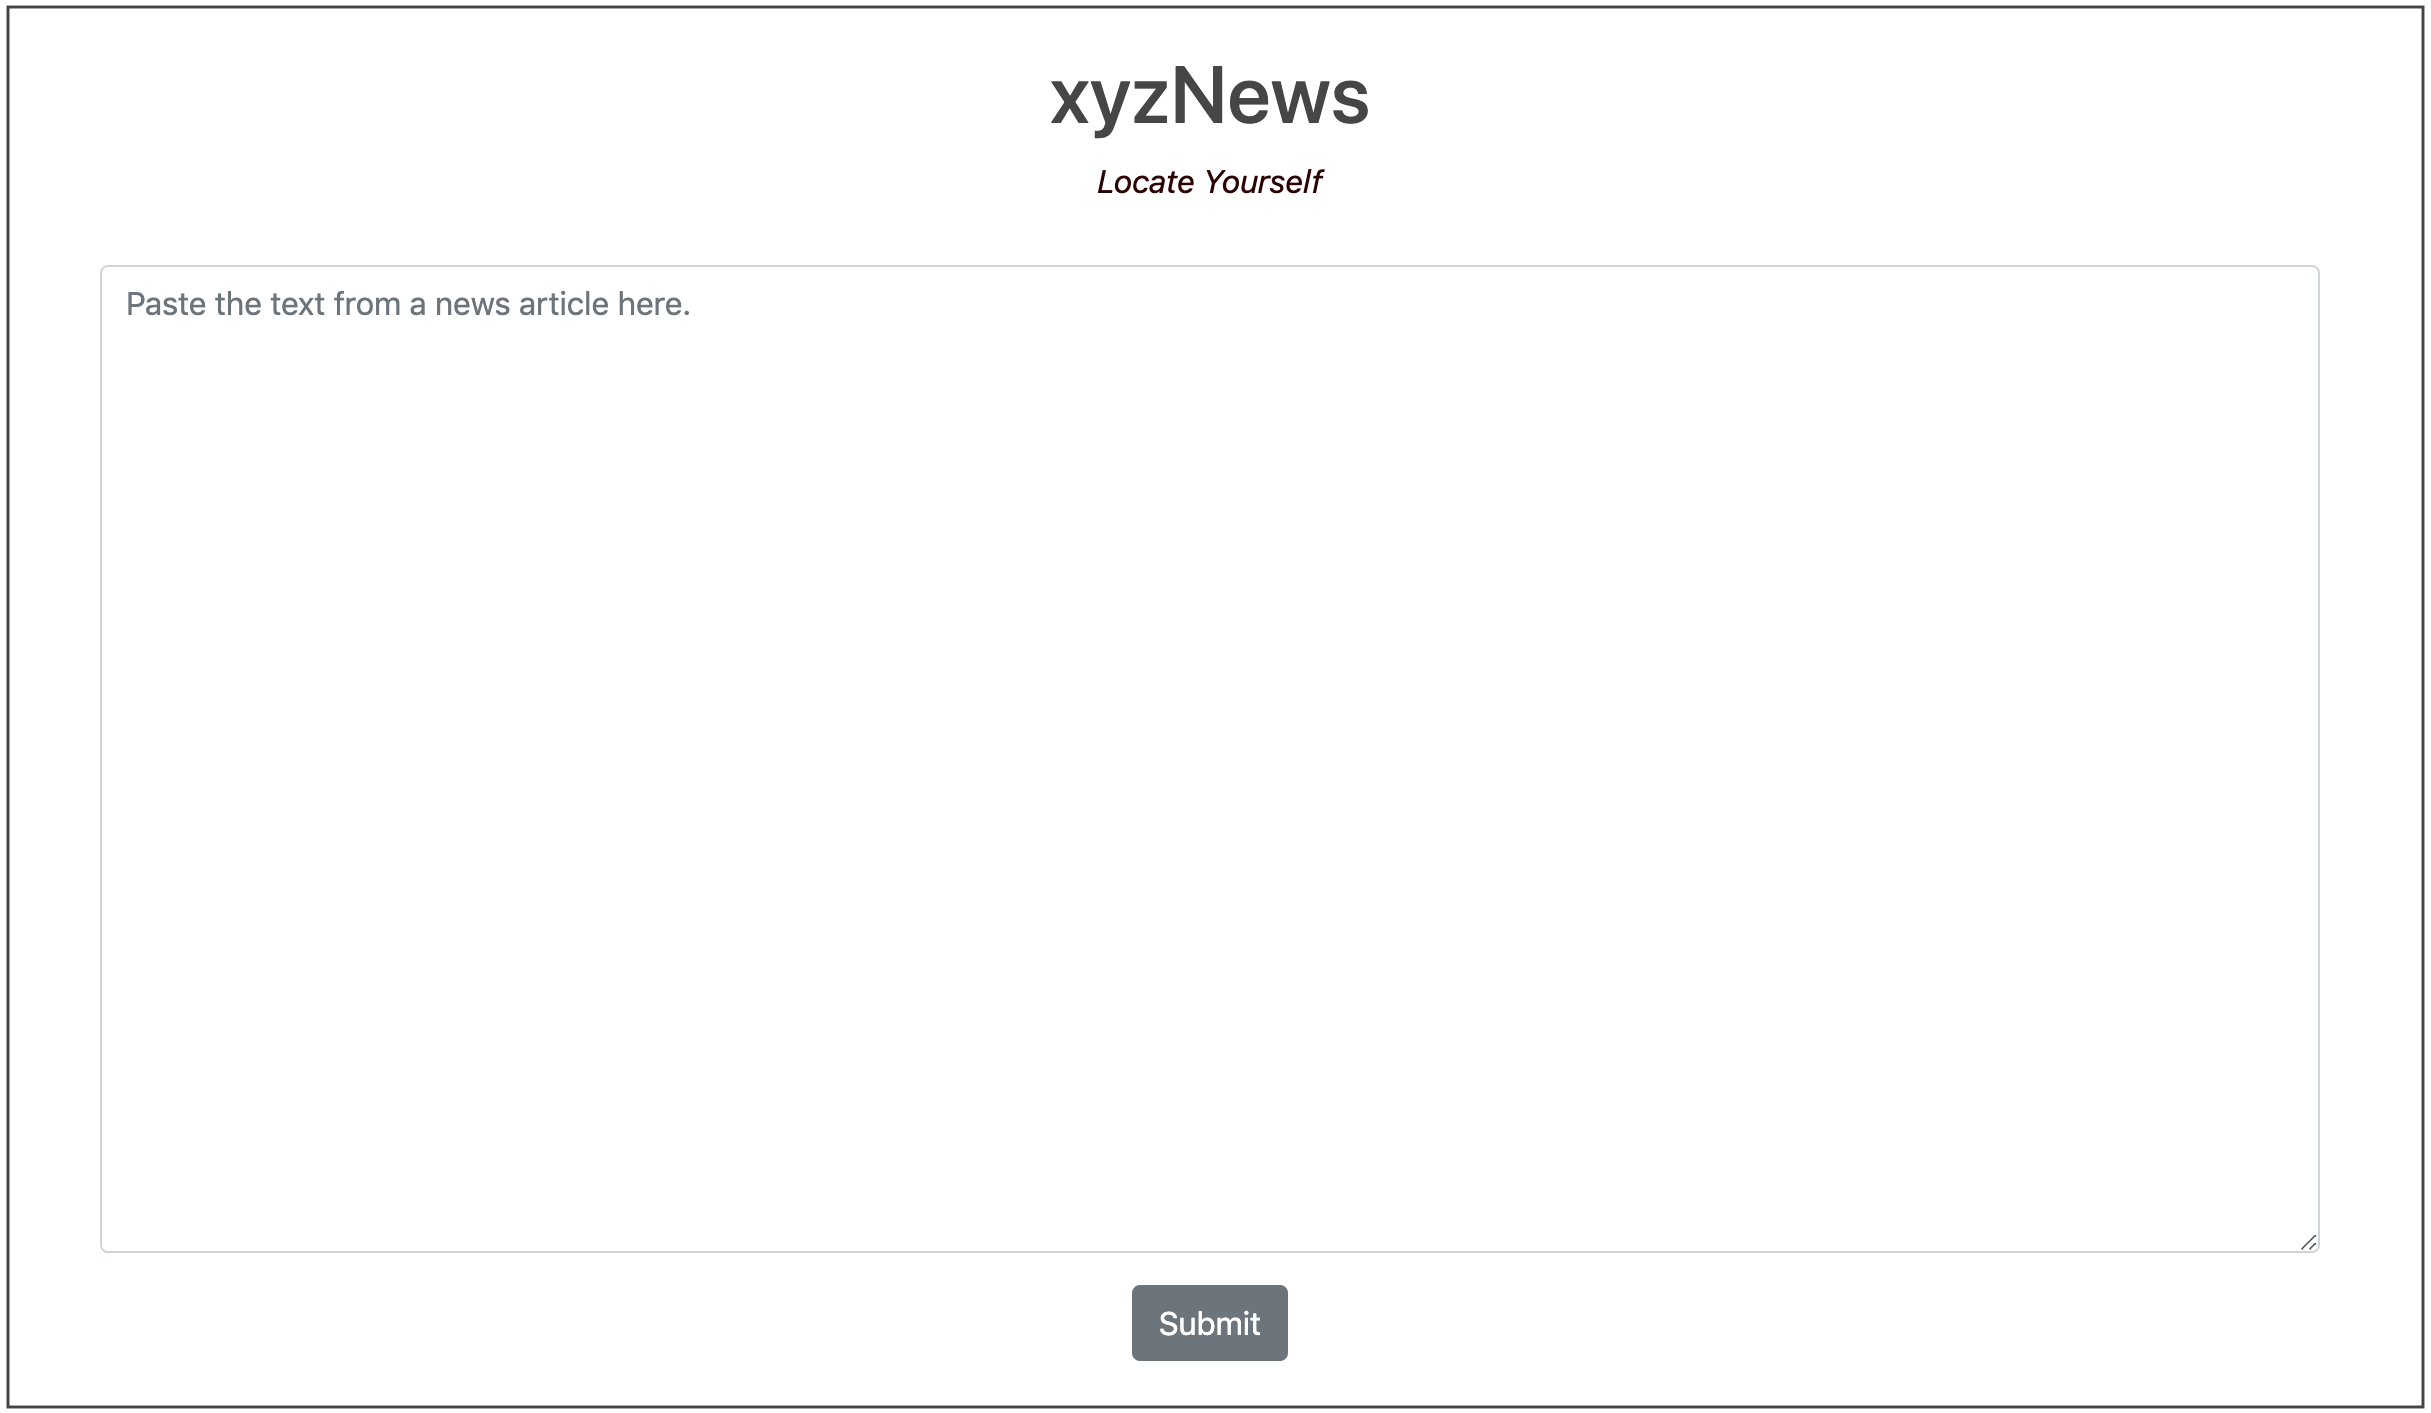
\includegraphics[width=\textwidth]{figures/images/web-form.png}
    		\caption{The web app;s home page.}
    		\label{fig:form}
    	\end{figure}
    \end{frame}


%%%%%%%%%%%%%%%%%%%%%%%%%%%%%%%%%%%%%%%%%%%%%%%%
% CONCLUSION 

\section{Conclusion and Discussion}

     \begin{frame}
    	\frametitle{Conclusion and Discussion}
    	\begin{itemize}
    		\item I've shown that NLP techniques can accurately classify news articles based on language differences in the underlying news sources. 
    		\item Given \citet{gentzkow2008competition} and \citet{gentzkow2006media}, it seems unlikely that biased news (or even fake news) will disappear anytime soon. 
    		\item A web application based on these ideas could serve as a starting point to measure news consumption. Analogus to: 
    		\begin{itemize}
    			\item Calendars can help to measure our time use.
    			\item Nutrition apps measure our macronutrients. 
    			\item GPS measures our geographical position.
    			\item Can we have an app to measure our news consumption? 
    		\end{itemize} 
    	\end{itemize}
    \end{frame}

    \begin{frame}
    	\frametitle{End}
    	\centering \Huge Thank you for your time.
    	
    	\centering Questions?
    \end{frame}

%%%%%%%%%%%%%%%%%%%%%%%%%%%%%%%%%%%%%%%%%%%%%%%%
% REFERENCES

\section{References}
    \begin{frame}
    	\frametitle{References}
    	\bibliographystyle{plainnat}
    	\bibliography{references/ref}
    \end{frame}


\end{document}